% 原PDF矢量路径与精确点位转为可编辑TikZ；未模拟点位。
\definecolor{chSevenADPlot5C0}{rgb}{0.136690,0.121950,0.125292}
\definecolor{chSevenADPlot5C1}{rgb}{0.286748,0.497444,0.740063}
\definecolor{chSevenADPlot5C2}{rgb}{0.218204,0.367498,0.543938}
\definecolor{chSevenADPlot5C3}{rgb}{0.305257,0.508278,0.748669}
\resizebox{.74\linewidth}{!}{
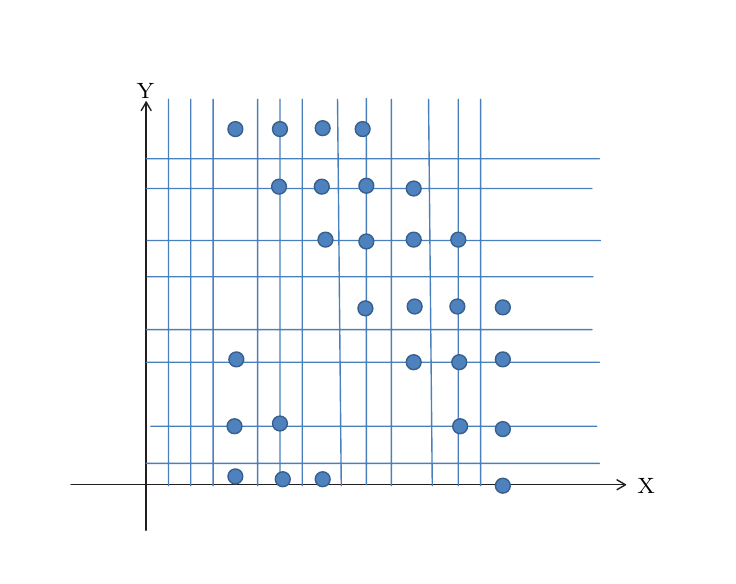
\begin{tikzpicture}[x=1bp,y=-1bp,line cap=round,line join=round]
\path[use as bounding box] (0,0) rectangle (245.00000,190.00000);
\path[line width=0.5000bp,draw=chSevenADPlot5C0,fill=none] (15.59700,164.55099) --(215.19199,164.55099);
\path[line width=0.5000bp,draw=chSevenADPlot5C0,fill=none] (212.14200,162.77197) --(215.19199,164.55099) --(212.14200,166.32898);
\path[line width=0.5000bp,draw=chSevenADPlot5C0,fill=none] (42.66499,180.92099) --(42.66499,26.79498);
\path[line width=0.5000bp,draw=chSevenADPlot5C0,fill=none] (44.44299,29.84399) --(42.66499,26.79498) --(40.88600,29.84399);
\path[line width=0.5000bp,draw=chSevenADPlot5C1,fill=none] (42.67799,120.43198) --(205.83301,120.43198) (43.02499,76.62097) --(206.17999,76.62097) (42.67799,47.20001) --(205.83301,47.20001) (58.72600,25.80298) --(58.72600,164.88498) (90.82300,25.80298) --(90.82300,164.88498) (121.92799,25.48199) --(121.92799,164.56400) (155.01401,25.80298) --(155.01401,164.88498) (42.67799,156.86099) --(205.83301,156.86099) (44.36301,143.48798) --(204.84399,143.48798) (42.67799,108.71698) --(203.15900,108.71698) (43.02499,89.67398) --(203.50601,89.67398) (42.67799,57.89899) --(203.15900,57.89899) (50.70200,25.80298) --(50.70200,164.88498) (66.75000,25.80298) --(66.75000,164.88498) (82.79800,25.80298) --(82.79800,164.88498) (98.84599,25.80298) --(98.84599,164.88498) (111.55099,25.80298) --(112.88901,164.88498) (130.94200,25.80298) --(130.94200,164.88498) (144.31599,25.80298) --(145.65300,164.88498) (163.03900,25.80298) --(163.03900,164.88498);
\path[line width=0.5000bp,draw=chSevenADPlot5C2,fill=chSevenADPlot5C3] (72.09900,36.50098) .. controls (72.09900,35.02399) and (73.29700,33.82599) .. (74.77400,33.82599) .. controls (76.25101,33.82599) and (77.44901,35.02399) .. (77.44901,36.50098) .. controls (77.44901,37.97900) and (76.25101,39.17596) .. (74.77400,39.17596) .. controls (73.29700,39.17596) and (72.09900,37.97900) .. (72.09900,36.50098) --cycle;
\path[line width=0.5000bp,draw=chSevenADPlot5C2,fill=chSevenADPlot5C3] (87.82600,57.22998) .. controls (87.82600,55.75299) and (89.02400,54.55499) .. (90.50101,54.55499) .. controls (91.97800,54.55499) and (93.17599,55.75299) .. (93.17599,57.22998) .. controls (93.17599,58.70697) and (91.97800,59.90399) .. (90.50101,59.90399) .. controls (89.02400,59.90399) and (87.82600,58.70697) .. (87.82600,57.22998) --cycle;
\path[line width=0.5000bp,draw=chSevenADPlot5C2,fill=chSevenADPlot5C3] (88.14799,36.50098) .. controls (88.14799,35.02399) and (89.34500,33.82599) .. (90.82300,33.82599) .. controls (92.30000,33.82599) and (93.49699,35.02399) .. (93.49699,36.50098) .. controls (93.49699,37.97900) and (92.30000,39.17596) .. (90.82300,39.17596) .. controls (89.34500,39.17596) and (88.14799,37.97900) .. (88.14799,36.50098) --cycle;
\path[line width=0.5000bp,draw=chSevenADPlot5C2,fill=chSevenADPlot5C3] (89.16400,162.55899) .. controls (89.16400,161.08099) and (90.36200,159.88397) .. (91.83800,159.88397) .. controls (93.31599,159.88397) and (94.51199,161.08099) .. (94.51199,162.55899) .. controls (94.51199,164.03598) and (93.31599,165.23297) .. (91.83800,165.23297) .. controls (90.36200,165.23297) and (89.16400,164.03598) .. (89.16400,162.55899) --cycle;
\path[line width=0.5000bp,draw=chSevenADPlot5C2,fill=chSevenADPlot5C3] (103.20599,57.22998) .. controls (103.20599,55.75299) and (104.40300,54.55499) .. (105.88000,54.55499) .. controls (107.35800,54.55499) and (108.55499,55.75299) .. (108.55499,57.22998) .. controls (108.55499,58.70697) and (107.35800,59.90399) .. (105.88000,59.90399) .. controls (104.40300,59.90399) and (103.20599,58.70697) .. (103.20599,57.22998) --cycle;
\path[line width=0.5000bp,draw=chSevenADPlot5C2,fill=chSevenADPlot5C3] (153.00800,143.48798) .. controls (153.00800,142.01099) and (154.20599,140.81299) .. (155.68201,140.81299) .. controls (157.16000,140.81299) and (158.35699,142.01099) .. (158.35699,143.48798) .. controls (158.35699,144.96500) and (157.16000,146.16199) .. (155.68201,146.16199) .. controls (154.20599,146.16199) and (153.00800,144.96500) .. (153.00800,143.48798) --cycle;
\path[line width=0.5000bp,draw=chSevenADPlot5C2,fill=chSevenADPlot5C3] (118.90601,101.04099) .. controls (118.90601,99.56400) and (120.10300,98.36697) .. (121.58099,98.36697) .. controls (123.05701,98.36697) and (124.25600,99.56400) .. (124.25600,101.04099) .. controls (124.25600,102.51797) and (123.05701,103.71597) .. (121.58099,103.71597) .. controls (120.10300,103.71597) and (118.90601,102.51797) .. (118.90601,101.04099) --cycle;
\path[line width=0.5000bp,draw=chSevenADPlot5C2,fill=chSevenADPlot5C3] (72.44701,119.41599) .. controls (72.44701,117.93900) and (73.64400,116.74100) .. (75.12199,116.74100) .. controls (76.59900,116.74100) and (77.79700,117.93900) .. (77.79700,119.41599) .. controls (77.79700,120.89398) and (76.59900,122.09000) .. (75.12199,122.09000) .. controls (73.64400,122.09000) and (72.44701,120.89398) .. (72.44701,119.41599) --cycle;
\path[line width=0.5000bp,draw=chSevenADPlot5C2,fill=chSevenADPlot5C3] (136.63901,100.37198) .. controls (136.63901,98.89499) and (137.83701,97.69800) .. (139.31400,97.69800) .. controls (140.79201,97.69800) and (141.98900,98.89499) .. (141.98900,100.37198) .. controls (141.98900,101.84900) and (140.79201,103.04700) .. (139.31400,103.04700) .. controls (137.83701,103.04700) and (136.63901,101.84900) .. (136.63901,100.37198) --cycle;
\path[line width=0.5000bp,draw=chSevenADPlot5C2,fill=chSevenADPlot5C3] (103.52699,162.55899) .. controls (103.52699,161.08099) and (104.72400,159.88397) .. (106.20200,159.88397) .. controls (107.67900,159.88397) and (108.87601,161.08099) .. (108.87601,162.55899) .. controls (108.87601,164.03598) and (107.67900,165.23297) .. (106.20200,165.23297) .. controls (104.72400,165.23297) and (103.52699,164.03598) .. (103.52699,162.55899) --cycle;
\path[line width=0.5000bp,draw=chSevenADPlot5C2,fill=chSevenADPlot5C3] (119.25301,56.90900) .. controls (119.25301,55.43201) and (120.45100,54.23401) .. (121.92799,54.23401) .. controls (123.40500,54.23401) and (124.60201,55.43201) .. (124.60201,56.90900) .. controls (124.60201,58.38599) and (123.40500,59.58398) .. (121.92799,59.58398) .. controls (120.45100,59.58398) and (119.25301,58.38599) .. (119.25301,56.90900) --cycle;
\path[line width=0.5000bp,draw=chSevenADPlot5C2,fill=chSevenADPlot5C3] (136.29201,57.89899) .. controls (136.29201,56.42096) and (137.48801,55.22400) .. (138.96700,55.22400) .. controls (140.44299,55.22400) and (141.64101,56.42096) .. (141.64101,57.89899) .. controls (141.64101,59.37598) and (140.44299,60.57300) .. (138.96700,60.57300) .. controls (137.48801,60.57300) and (136.29201,59.37598) .. (136.29201,57.89899) --cycle;
\path[line width=0.5000bp,draw=chSevenADPlot5C2,fill=chSevenADPlot5C3] (104.54300,76.30096) .. controls (104.54300,74.82300) and (105.74100,73.62598) .. (107.21800,73.62598) .. controls (108.69501,73.62598) and (109.89301,74.82300) .. (109.89301,76.30096) .. controls (109.89301,77.77802) and (108.69501,78.97498) .. (107.21800,78.97498) .. controls (105.74100,78.97498) and (104.54300,77.77802) .. (104.54300,76.30096) --cycle;
\path[line width=0.5000bp,draw=chSevenADPlot5C2,fill=chSevenADPlot5C3] (103.52699,36.17999) .. controls (103.52699,34.70300) and (104.72400,33.50598) .. (106.20200,33.50598) .. controls (107.67900,33.50598) and (108.87601,34.70300) .. (108.87601,36.17999) .. controls (108.87601,37.65698) and (107.67900,38.85498) .. (106.20200,38.85498) .. controls (104.72400,38.85498) and (103.52699,37.65698) .. (103.52699,36.17999) --cycle;
\path[line width=0.5000bp,draw=chSevenADPlot5C2,fill=chSevenADPlot5C3] (117.91600,36.50098) .. controls (117.91600,35.02399) and (119.11400,33.82599) .. (120.59200,33.82599) .. controls (122.06799,33.82599) and (123.26500,35.02399) .. (123.26500,36.50098) .. controls (123.26500,37.97900) and (122.06799,39.17596) .. (120.59200,39.17596) .. controls (119.11400,39.17596) and (117.91600,37.97900) .. (117.91600,36.50098) --cycle;
\path[line width=0.5000bp,draw=chSevenADPlot5C2,fill=chSevenADPlot5C3] (119.25301,76.96899) .. controls (119.25301,75.49200) and (120.45100,74.29401) .. (121.92799,74.29401) .. controls (123.40500,74.29401) and (124.60201,75.49200) .. (124.60201,76.96899) .. controls (124.60201,78.44598) and (123.40500,79.64398) .. (121.92799,79.64398) .. controls (120.45100,79.64398) and (119.25301,78.44598) .. (119.25301,76.96899) --cycle;
\path[line width=0.5000bp,draw=chSevenADPlot5C2,fill=chSevenADPlot5C3] (136.29201,76.30096) .. controls (136.29201,74.82300) and (137.48801,73.62598) .. (138.96700,73.62598) .. controls (140.44299,73.62598) and (141.64101,74.82300) .. (141.64101,76.30096) .. controls (141.64101,77.77802) and (140.44299,78.97498) .. (138.96700,78.97498) .. controls (137.48801,78.97498) and (136.29201,77.77802) .. (136.29201,76.30096) --cycle;
\path[line width=0.5000bp,draw=chSevenADPlot5C2,fill=chSevenADPlot5C3] (152.34000,76.30096) .. controls (152.34000,74.82300) and (153.53700,73.62598) .. (155.01401,73.62598) .. controls (156.49100,73.62598) and (157.68900,74.82300) .. (157.68900,76.30096) .. controls (157.68900,77.77802) and (156.49100,78.97498) .. (155.01401,78.97498) .. controls (153.53700,78.97498) and (152.34000,77.77802) .. (152.34000,76.30096) --cycle;
\path[line width=0.5000bp,draw=chSevenADPlot5C2,fill=chSevenADPlot5C3] (152.01801,100.37198) .. controls (152.01801,98.89499) and (153.21600,97.69800) .. (154.69299,97.69800) .. controls (156.17099,97.69800) and (157.36801,98.89499) .. (157.36801,100.37198) .. controls (157.36801,101.84900) and (156.17099,103.04700) .. (154.69299,103.04700) .. controls (153.21600,103.04700) and (152.01801,101.84900) .. (152.01801,100.37198) --cycle;
\path[line width=0.5000bp,draw=chSevenADPlot5C2,fill=chSevenADPlot5C3] (168.38800,100.69299) .. controls (168.38800,99.21597) and (169.58499,98.01898) .. (171.06299,98.01898) .. controls (172.54001,98.01898) and (173.73801,99.21597) .. (173.73801,100.69299) .. controls (173.73801,102.17099) and (172.54001,103.36798) .. (171.06299,103.36798) .. controls (169.58499,103.36798) and (168.38800,102.17099) .. (168.38800,100.69299) --cycle;
\path[line width=0.5000bp,draw=chSevenADPlot5C2,fill=chSevenADPlot5C3] (71.77800,143.48798) .. controls (71.77800,142.01099) and (72.97600,140.81299) .. (74.45300,140.81299) .. controls (75.92999,140.81299) and (77.12801,142.01099) .. (77.12801,143.48798) .. controls (77.12801,144.96500) and (75.92999,146.16199) .. (74.45300,146.16199) .. controls (72.97600,146.16199) and (71.77800,144.96500) .. (71.77800,143.48798) --cycle;
\path[line width=0.5000bp,draw=chSevenADPlot5C2,fill=chSevenADPlot5C3] (168.38800,164.88498) .. controls (168.38800,163.40900) and (169.58499,162.20999) .. (171.06299,162.20999) .. controls (172.54001,162.20999) and (173.73801,163.40900) .. (173.73801,164.88498) .. controls (173.73801,166.36298) and (172.54001,167.56000) .. (171.06299,167.56000) .. controls (169.58499,167.56000) and (168.38800,166.36298) .. (168.38800,164.88498) --cycle;
\path[line width=0.5000bp,draw=chSevenADPlot5C2,fill=chSevenADPlot5C3] (136.29201,120.43198) .. controls (136.29201,118.95499) and (137.48801,117.75699) .. (138.96700,117.75699) .. controls (140.44299,117.75699) and (141.64101,118.95499) .. (141.64101,120.43198) .. controls (141.64101,121.90997) and (140.44299,123.10699) .. (138.96700,123.10699) .. controls (137.48801,123.10699) and (136.29201,121.90997) .. (136.29201,120.43198) --cycle;
\path[line width=0.5000bp,draw=chSevenADPlot5C2,fill=chSevenADPlot5C3] (152.68700,120.43198) .. controls (152.68700,118.95499) and (153.88499,117.75699) .. (155.36200,117.75699) .. controls (156.84000,117.75699) and (158.03699,118.95499) .. (158.03699,120.43198) .. controls (158.03699,121.90997) and (156.84000,123.10699) .. (155.36200,123.10699) .. controls (153.88499,123.10699) and (152.68700,121.90997) .. (152.68700,120.43198) --cycle;
\path[line width=0.5000bp,draw=chSevenADPlot5C2,fill=chSevenADPlot5C3] (168.38800,119.41599) .. controls (168.38800,117.93900) and (169.58499,116.74100) .. (171.06299,116.74100) .. controls (172.54001,116.74100) and (173.73801,117.93900) .. (173.73801,119.41599) .. controls (173.73801,120.89398) and (172.54001,122.09000) .. (171.06299,122.09000) .. controls (169.58499,122.09000) and (168.38800,120.89398) .. (168.38800,119.41599) --cycle;
\path[line width=0.5000bp,draw=chSevenADPlot5C2,fill=chSevenADPlot5C3] (88.14799,142.49799) .. controls (88.14799,141.02100) and (89.34500,139.82397) .. (90.82300,139.82397) .. controls (92.30000,139.82397) and (93.49699,141.02100) .. (93.49699,142.49799) .. controls (93.49699,143.97598) and (92.30000,145.17297) .. (90.82300,145.17297) .. controls (89.34500,145.17297) and (88.14799,143.97598) .. (88.14799,142.49799) --cycle;
\path[line width=0.5000bp,draw=chSevenADPlot5C2,fill=chSevenADPlot5C3] (168.38800,144.50497) .. controls (168.38800,143.02698) and (169.58499,141.82999) .. (171.06299,141.82999) .. controls (172.54001,141.82999) and (173.73801,143.02698) .. (173.73801,144.50497) .. controls (173.73801,145.98199) and (172.54001,147.17999) .. (171.06299,147.17999) .. controls (169.58499,147.17999) and (168.38800,145.98199) .. (168.38800,144.50497) --cycle;
\path[line width=0.5000bp,draw=chSevenADPlot5C2,fill=chSevenADPlot5C3] (72.09900,161.54099) .. controls (72.09900,160.06497) and (73.29700,158.86798) .. (74.77400,158.86798) .. controls (76.25101,158.86798) and (77.44901,160.06497) .. (77.44901,161.54099) .. controls (77.44901,163.01999) and (76.25101,164.21698) .. (74.77400,164.21698) .. controls (73.29700,164.21698) and (72.09900,163.01999) .. (72.09900,161.54099) --cycle;
\node[inner sep=0pt,font=\fontsize{8}{9}\selectfont] at (222.62875,164.99533) {$\mathrm{X}$};
\node[inner sep=0pt,font=\fontsize{8}{9}\selectfont] at (42.53423,22.62335) {$\mathrm{Y}$};
\end{tikzpicture}
}
